\documentclass[11pt]{amsart}
\usepackage{geometry}                % See geometry.pdf to learn the layout options. There are lots.
\geometry{letterpaper}                   % ... or a4paper or a5paper or ... 
\usepackage[parfill]{parskip}    % Activate to begin paragraphs with an empty line rather than an indent
\usepackage{graphicx}
\usepackage{amssymb}
\usepackage[ngerman]{babel}
\theoremstyle{remark}
\usepackage{epstopdf}
\makeindex

\title{Analysis I}
\author{Daniel Roth}
\date{\today}

\begin{document}

\begin{titlepage}
\maketitle
\begin{table}[b]
\begin{center}
Version 0.1\_1
\end{center}
\end{table}
\end{titlepage}

\tableofcontents
\newpage
\section{Einleitung}
\subsection{Lizenz}
Dieses Werk ist unter einem Creative Commons Namensnennung-Weitergabe unter gleichen Bedingungen 3.0 Unported Lizenzvertrag lizenziert. Um die Lizenz anzusehen, gehen Sie bitte zu http://creativecommons.org/licenses/by-sa/3.0/ oder schicken Sie einen Brief an Creative Commons, 171 Second Street, Suite 300, San Francisco, California 94105, USA.

\section{Grenzwert von Folgen und Funktionen}
Buch Seiten
\\Formelsammlung Seiten
\subsection{Grenzwerte von Zahlenfolgen}
\textbf{ \\Definition:} Unter einer \underline{reellen Zahlenfolge}\index{reellen Zahlenfolge}\index{reellen}\index{Zahlenfolge} versteht man eine \underline{geordnete}\index{geordnete} Menge reeller Zahlen.\\
\textbf{Schreibweise}:$\langle a_n\rangle n\in\mathbb{N}= a_1, a_2, a_3, \dotsb, a_n$\\
Die Zahlen $a_1,a_2,a_3, \dotsb , a_n$ heissen \underline{Glieder}\index{Glieder} der Folge. \\$a_n : \text{n-test Glied der Folge}$, wobei $n$ jeweils mit $1$ beginnt.
\subsubsection*{Beispiele:}
\begin{equation}
\langle a_n\rangle n\in\mathbb{N} =-\frac{1}{2}, -\frac{1}{4}, -\frac{1}{6}, \dotsb \\\text{Das heisst,} a_n=-\frac{1}{2n} , n \in\mathbb{N}
\end{equation}
\begin{equation}
\langle a_n\rangle n\in\mathbb{N} =1^3, 2^3, 3^3, \dotsb \\\text{Das heisst,} a_n=n^3, n \in\mathbb{N}
\end{equation}
\begin{equation}
\langle a_n\rangle n\in\mathbb{N} =0, \frac 12, \frac 23, \frac 34, \dotsb \\\text{Das heisst,} a_n=1-\frac 1n, n \in\mathbb{N}
\end{equation}
\subsubsection*{Darstellung:}
Die anschaulichste Darstellung einer Folge ist ein \underline{Graph}\index{Graph}. Wir ordnen jedem Wertepaar $(n, a_n) n \in\mathbb{N}$ einen Punkt, im Koordinatensystem zu.
\newpage
\subsubsection*{Beispiel:}
\begin{center}
Wir betrachten nochmals $\langle a_n \rangle_{n \in \mathbb{N}} = 1 - \frac 1n$\\
\begin{figure}[h]
  \centering
  \fbox{
    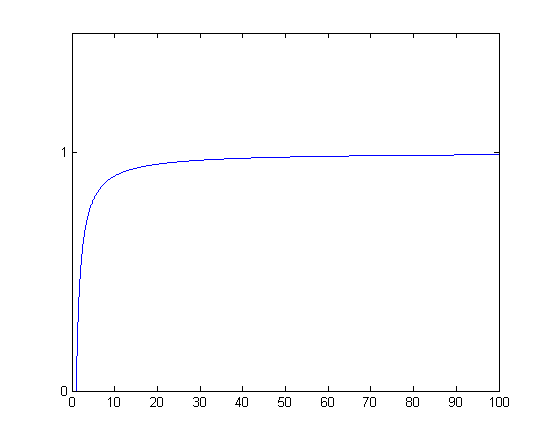
\includegraphics[width=15cm]{figures/figure1.png}
    }
 \end{figure}
\begin{table}[h]
\caption{Folge des Graphs}
\begin{tabular}[t]{lrrrrrrrrrr}
n & 1 & 2 & 3 & 4 & 5 & $\dotsb$ & 100& $\dotsb$ & 1000 & $\dotsb$ \\
$a_n$ & 0 & $\frac 12$ & $\frac 23$&$\frac 34$&$\frac 45$&$\dotsb$&$\frac {99}{100}$&$\dotsb$&$\frac {999}{1000}$&$\dotsb$\\
\end{tabular}
\label{default}
\end{table}
\end{center}
Man sagt: In jeder noch so kleinen Umgebung von 1 liegen fast alle Glieder der Folge $\langle a_n\rangle = 1 -\frac 1n n \in \mathbb{N}$
\subsubsection*{Definition:}
Eine Folge heisst \underline{konvergent}\index{konvergent}, wenn sie einen \underline{Grenzwert}\index{Grenzwert} g besitzt.\\
\textbf{Schreibweise:} $\lim_{n \to \infty}x_n = g$ (Limes von $a_n$ f\"{u}r $n$ gegen $\infty $ ist gleich $g$. $g \in \mathbb{R} \setminus \lbrace \pm\infty \rbrace$
Besitzt die Folge keinen Grenzwert, so ist sie \underline{divergent}\index{divergent}.
\subsubsection*{Beispiele:} 
\begin{equation}
	{\langle a_n\rangle}_{n \in \mathbb{N}} ={\langle \frac {1}{n} \rangle}_{n \in \mathbb{N}} = 1, \frac{1}{2}, \frac 13, \dotsb 
\end{equation}
\begin{equation*}
 \lim_{n \to \infty} ( \frac 1n )_{n \in \mathbb{N}} = g = 0
\end{equation*}
\begin{equation*}	
	\text{konvergiert gegen } 0
\end{equation*}
\begin{equation}
	{\langle a_n\rangle}_{n \in \mathbb{N}} ={\langle 1-\frac {1}{n} \rangle}_{n \in \mathbb{N}} 
\end{equation}
\begin{equation*}
g = 1 = \lim_{n \to \infty} ( 1- \frac 1n )_{n \in \mathbb{N}}
\end{equation*}
\begin{equation*}	
	\text{konvergiert gegen } 1
\end{equation*}
\begin{equation}
	{\langle a_n\rangle}_{n \in \mathbb{N}} ={\langle 1+(\frac {1}{n})^n \rangle}_{n \in \mathbb{N}} = 2, \frac{9}{4}, \frac {64}{27}, \dotsb 
\end{equation}
\begin{equation*}
g = e = \lim_{n \to \infty} (1+ (\frac 1n)^n )_{n \in \mathbb{N}}
\end{equation*}
\begin{equation*}	
	\text{konvergiert gegen } e
\end{equation*}
\begin{equation}
	{\langle a_n\rangle}_{n \in \mathbb{N}} ={\langle n^3 \rangle}_{n \in \mathbb{N}} = 1,8,27, \dotsb 
\end{equation}
\begin{equation*}
g = \infty = \lim_{n \to \infty} (1+ (\frac 1n)^n )_{n \in \mathbb{N}}
\end{equation*}
\begin{equation*}	
	\text{divergiert gegen } \infty \text{, das heisst uneigentlicher Grenzwert}
\end{equation*}

\subsection{Grenzwert einer Funktion $f(x)$ f\"ur $x 	\to x_0$}
\subsubsection*{Definition:}
Sei $f(x) = y$ in einer Umgebung von $x_0$ definiert (in $x_0$ selber muss sie nicht definiert sein). Gilt dann f\"ur die Folge $x_n \xrightarrow{n \to \infty} x_0$, dass $f(x_n) \xrightarrow[n \to \infty]{} (f(x_0) = g)$ also $\lim_{n \to \infty} (f(x_n)) = g$ , so heisst \underline{g der Grenzwert}\index{Grenzwert} von $f(x)$ an der Stelle $x_0$.\\
\begin{equation*}
\lim_{x \to x_0} f(x) = g
\end{equation*}
\subsubsection*{Beispiele:} 
\begin{equation}
	f(x) = \frac{x^2 - x -12}{x+3} = \frac{(x-4)(x+3)}{x+3} = x-4
\end{equation}
\begin{equation*}
	x_0 = -3
\end{equation*}
\begin{equation*}
	\lim_{x \to -3} \left(\frac{x^2-x-12}{x+3}\right) = \lim_{x \to -3} (x-4) = -7
\end{equation*}
\begin{figure}[h]
  \centering
  \fbox{
    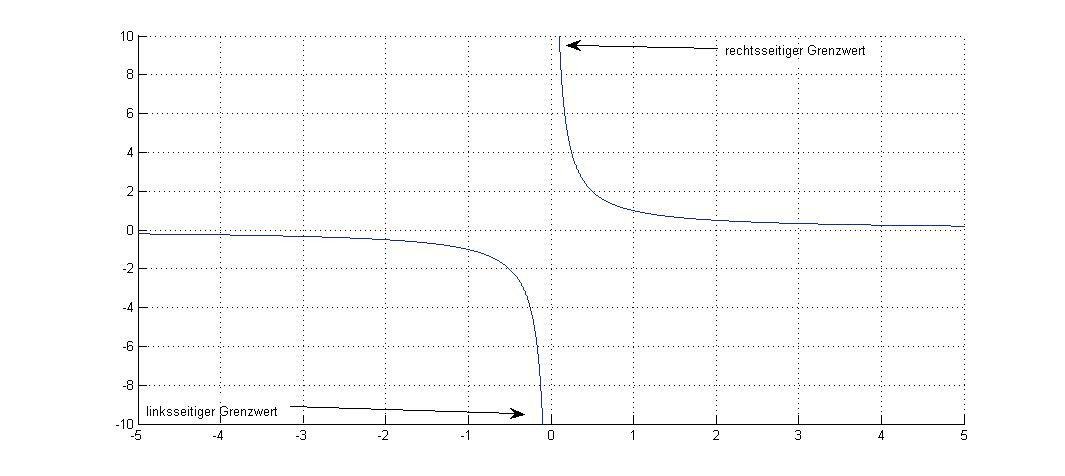
\includegraphics[width=15cm]{figures/figure2.jpg}
    }
 \end{figure}
\begin{equation}
	f(x) = \frac 1x 
\end{equation}
\begin{equation*}
	x_0 = 0
\end{equation*}
\begin{equation*}
	\lim_{x \to 0} \frac 1x = \text{kein Grenzwert f\"ur $x \to 0$}
\end{equation*}
\begin{equation*}
	\text{linksseitiger Grenzwert}\lim_{x \uparrow 0} f(x) = -\infty
\end{equation*}
\begin{equation*}
	\text{rechtsseitiger Grenzwert}\lim_{x \downarrow 0} f(x) = \infty
\end{equation*}
\subsubsection*{Problem:}
Linksseitiger Grenzwert $\ne$ rechtsseitiger Grenzwert $\Rightarrow \frac 1x$ besitzt \underline{keinen} Grenzwert an der Stelle $x_0$.
\subsubsection*{Es gilt:\\}
Besitzt $f(x)$ an der Stelle $x_0$ einen Grenzwert $g$, so ist :
\begin{equation}
\lim_{x \uparrow x_0} f(x) = -\infty = \lim_{x \downarrow x_0} f(x) = -\infty \lim_{x \to x_0} f(x) = -\infty
\end{equation}
\subsubsection*{Beispiele:}

\begin{figure}[h]
  \centering
  \fbox{
    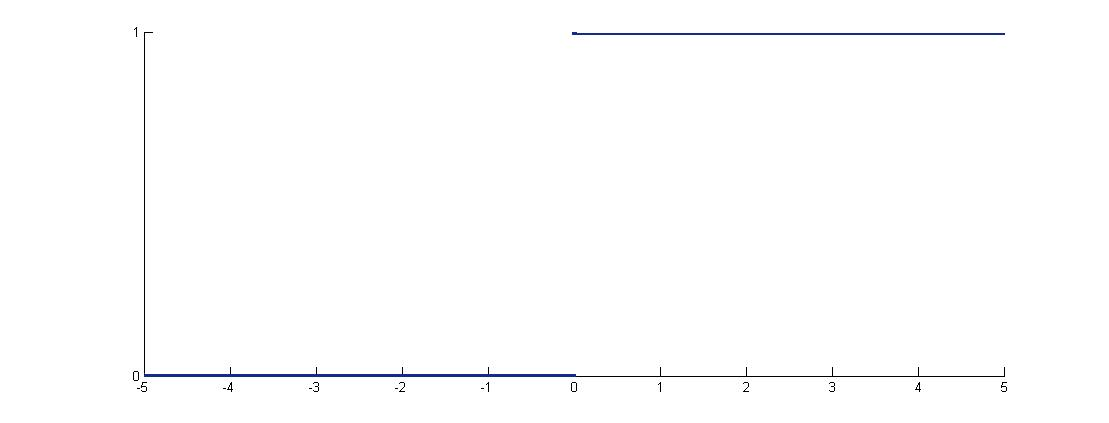
\includegraphics[width=15cm]{figures/figure3.jpg}
    }
 \end{figure}
\begin{equation}
f(x) =\left\lbrace \begin{array}{ccc}
  0 & , & x \langle	 0\\
  1 & , & x \rangle 0\\
\end{array}\right\rbrace
\end{equation}
\begin{equation*}
\lim_{x \to 0} f(x) \Rightarrow \text{kein Grenzwert}
\end{equation*}
\begin{equation*}
\lim_{x \downarrow 0} f(x) = 1
\end{equation*}
\begin{equation*}
\lim_{x \uparrow 0} f(x) = 0
\end{equation*}
\begin{figure}[h]
  \centering
  \fbox{
    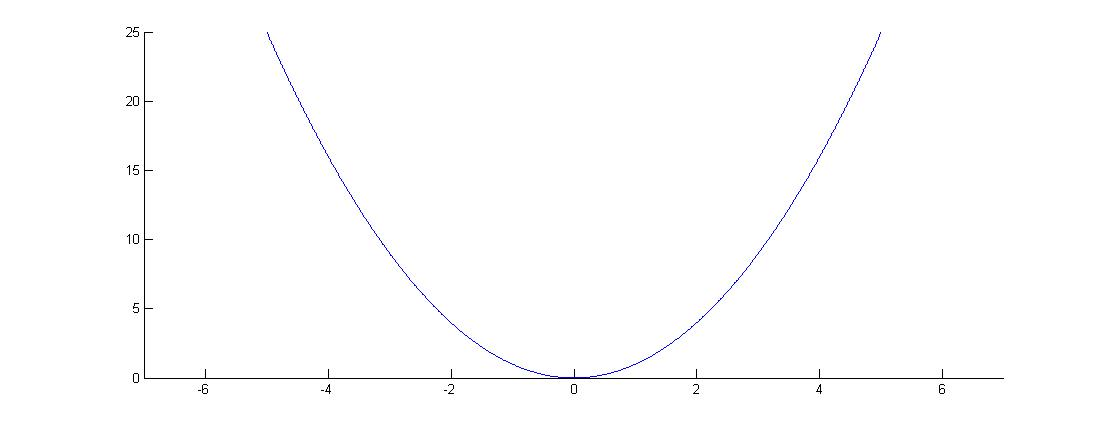
\includegraphics[width=15cm]{figures/figure4.jpg}
    }
 \end{figure}\begin{equation}
f(x) = x^2
\end{equation}
\begin{equation*}
\lim_{x \to \pm2} f(x) = 4
\end{equation*}
\begin{equation*}
\lim_{x \downarrow \pm2} f(x) = 4
\end{equation*}
\begin{equation*}
\lim_{x \uparrow \pm2} f(x) = 4
\end{equation*}

\subsection{Stetigkeit einer Funktion $f(x)$ in $x_0$}
Eine Funktion heisst \underline{stetig}\index{stetig} in $x_0$, wenn (beide Bedingungen m\"ussen erf\"ullt sein):\\
\begin{itemize}
\item[] \begin{equation*}
\lim_{x \uparrow x_o} f(x) = \lim_{x \downarrow x_0} f(x)
\end{equation*}
\item[] Der Grenzwert bei $x_0$ entspricht dem Funktionswert $f(x_0)$ (das heisst $f(x_0)$ ist definiert)\end{itemize}
\subsubsection*{Illustrativ:}
"Die Funktion kann ohne Absetzen des Stiftes gezeichnet werden."
\subsection{Der Grenzwert einer Funktion $f(x)$, $x\to\pm\infty$}
\begin{figure}[h]
  \centering
  \fbox{
    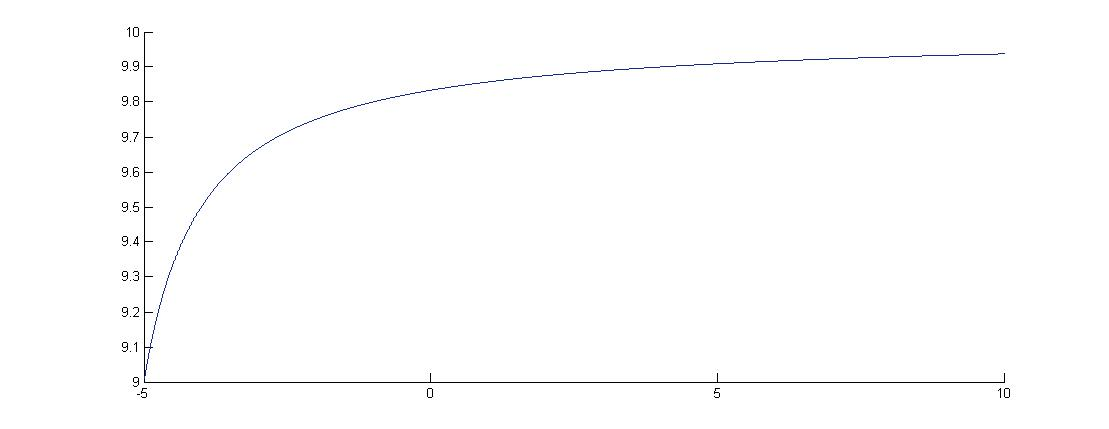
\includegraphics[width=15cm]{figures/figure5.jpg}
    }
 \end{figure}
steigt die Funktion beliebig weiter?\\\\
Um diese Frage zu beantworten, brauchen wir $\lim_{x\to\infty} f(x)$.
\subsubsection*{Beispiele:}
\begin{equation}
\lim_{x\to\infty} \frac 1x = 0
\end{equation}
\begin{equation}
\lim_{x\to\infty} \frac {x^3}{x^2+2} = \infty \text{(die h\"ohere Potenz ist st\"arker)}
\end{equation}
\begin{equation}
\lim_{x\to\infty} \frac {e^x}{x^3} = \infty \text{($e^x$ ist st\"arker als jede Potenz von x)}
\end{equation}
\begin{equation}
\lim_{x\to\infty} \frac {\ln x}{x^2} = \infty \text{($\ln x$ ist schw\"acher als jede Potenz von x)}
\end{equation}

\subsection{Erg\"anzung:Grenzwert einer Funktion}
Die Regel von Bernoulli de l'H\^opital.\\
Betrachte Grenzwerte vom Typ
\begin{equation*}
\lim_{x \to \infty} \frac {f(x)}{g(x)} \text{,} \lim_{x \to x_0} \frac {f(x)}{g(x)}
\end{equation*}
die auf einen unbestimmten Ausdruck wie zum Beispiel $\frac 00$,$\frac \infty\infty$ oder $\frac {-\infty}\infty$ f\"uhren. \\
Solche Grenzwerte (und nur solche) k\"onnen mit der Regel von Bernoulli de l'H\^opital bestimmt werden.
\begin{equation}
\lim_{x \to x_0} \frac {f(x)}{g(x)} = \lim_{x \to x_0} \frac {f'(x)}{g'(x)}
\end{equation}
\begin{equation*}
\lim_{x \to \pm\infty} \frac {f(x)}{g(x)} = \lim_{x \to \pm\infty} \frac {f'(x)}{g'(x)}
\end{equation*}
\subsubsection*{Beispiele}
\begin{equation}
\lim_{x \to 0}\left(\frac {e^x-1}{x}\right) = \lim_{x \to 0}\frac {f(x)}{g(x)}=\frac 00
\end{equation}
\begin{equation*}
\text{also:} \lim_{x \to 0}\frac {f(x)}{g(x)}\overset {\text{BdH}}{=} \lim_{x \to 0}\frac {f'(x)}{g'(x)} = \lim_{x \to 0} \frac {e^x}1 = 1
\end{equation*}

\newpage
\section{Differentialrechnung}
Buch\\
Formelsammlung\\
Besch\"aftigt sich mit der Frage: Wie ist der Kurvenverlauf einer Funktion?\\
Eckdaten:
\begin{itemize}
\item Definitionsl\"ucken
\item Nullstellen einer Funktion
\item[(*)]Steigung der Funktion in bestimmten Punkten
\item[(*)]Extremalstellen (Maxima/Minima)
\item[(*)]Wendepunkte
\end{itemize}
F\"ur die (*)-Begriffe ben\"otigen wir die \underline{Ableitung}\index{Ableitung}/ das \underline{Differential}\index{Differntial} einer Funktion.\\
Wir f\"uhren den Begriff der Ableitung mit Hilfe der Steigung einer Funktion ein.
\subsection{Das Tangentenproblem}
\begin{figure}[h]
  \centering
  \fbox{
    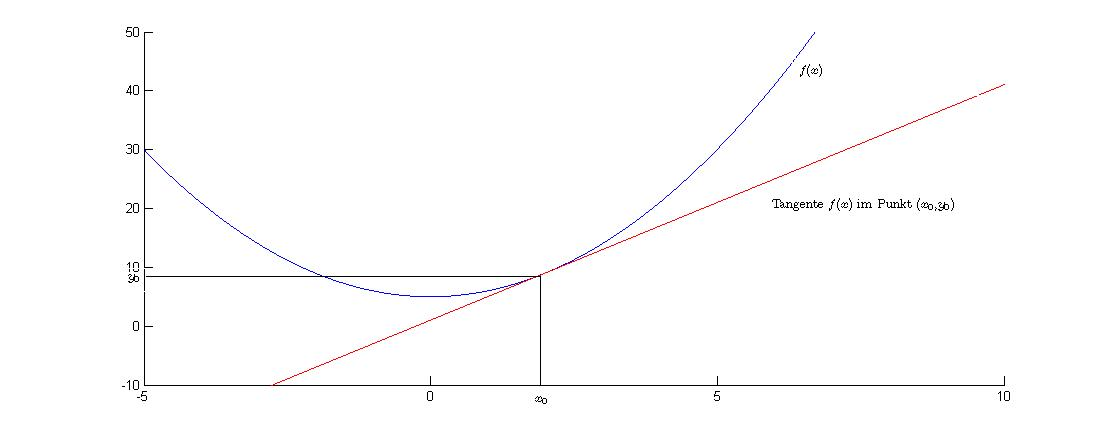
\includegraphics[width=15cm]{figures/figure6.jpg}
      }
 \end{figure}
\underline{Die Steigung der Funktion} $f(x)$ im Punkt $x_0$, ist identisch mit der \underline{Steigung der Tangente} an $f(x)$ in $x_0$
\subsubsection*{Problem:}
Um die Steigung der Tangente zu bestimmen brauchen wir einen \underline{2-ten} Punkt.
\subsubsection*{L\"osung:}
Zeichnen eine \underline{Sekante} und k\"onnen so die Steigung der Tangente herleiten.
\begin{figure}[h]
  \centering
  \fbox{
    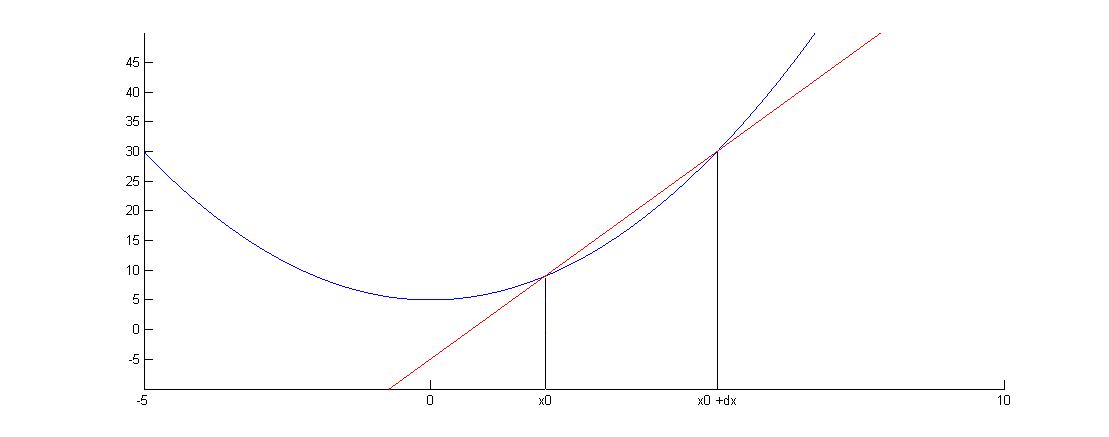
\includegraphics[width=15cm]{figures/figure7.jpg}
    }
 \end{figure}
Steigung der Sekante $= \frac {\mathrm dx}{\mathrm dy}=\frac {f(x_0 + \mathrm dx ) - f(x_0)}{\mathrm dx}$\newline
Steigung der \underline{Tangente}
\begin{equation*}
	\lim_{\mathrm dx \to \infty} \left( \frac {f(x_0 + \mathrm dx) - f(x_0)}{\mathrm dx} \right) = f'(x_0)
\end{equation*}
Verkleinere $\mathrm dx$ beliebig stark, das heisst $\mathrm dx \to 0$. \newline
$f'(x)$: erste Ableitung von $f(x)$ an der Stelle $x_0$.\newline
$\lim_{\mathrm dx \to \infty} \left( \frac {f(x_0 + \mathrm dx) - f(x_0)}{\mathrm dx} \right)$: ist der Differenzenquotient.
\subsubsection*{Beispiel(Diffrenzenquotient):}
\begin{equation}
	f(x) = a
\end{equation}
\begin{equation*}
	f'(x_0) = \lim_{\mathrm dx \to 0} \left( \frac {f(x_0 + \mathrm dx) - f(x_0)}{\mathrm dx} \right) = \lim_{\mathrm dx \to 0} \left( \frac {a-a}{\mathrm dx} \right)= 0
\end{equation*}
\begin{equation}
	f(x) = x
\end{equation}
\begin{equation*}
	f'(x_0) = \lim_{\mathrm dx \to 0} \left( \frac {f(x_0 + \mathrm dx) - f(x_0)}{\mathrm dx} \right) = \lim_{\mathrm dx \to 0} \left( \frac {\mathrm dx + x_0-x_0}{\mathrm dx} \right)= 1
\end{equation*}
\begin{equation}
	f(x) = x^2
\end{equation}
\begin{equation*}
	f'(x_0) = \lim_{\mathrm dx \to 0} \left( \frac {f(x_0 + \mathrm dx) - f(x_0)}{\mathrm dx} \right) =  
	\lim_{\mathrm dx \to 0} \left( \frac {(x_0 + \mathrm dx)^2 - (x_0)^2}{\mathrm dx} \right) =
	\end{equation*}
\begin{equation*}
	\lim_{\mathrm dx \to 0} \left( \frac { x_0^2 + 2x\mathrm dx + \mathrm dx^2 -x_0^2}{\mathrm dx} \right)= 
	2x_0
\end{equation*}

\subsection{Differenzierbareit von Funktionen}
Eine Funktion ist differnzierbar, wenn sich der Differenzenquotient berechnen l\"asst. Beispiele bei denen dies nicht funktioniert.\newline
\begin{figure}[h]
  \centering
  \fbox{
    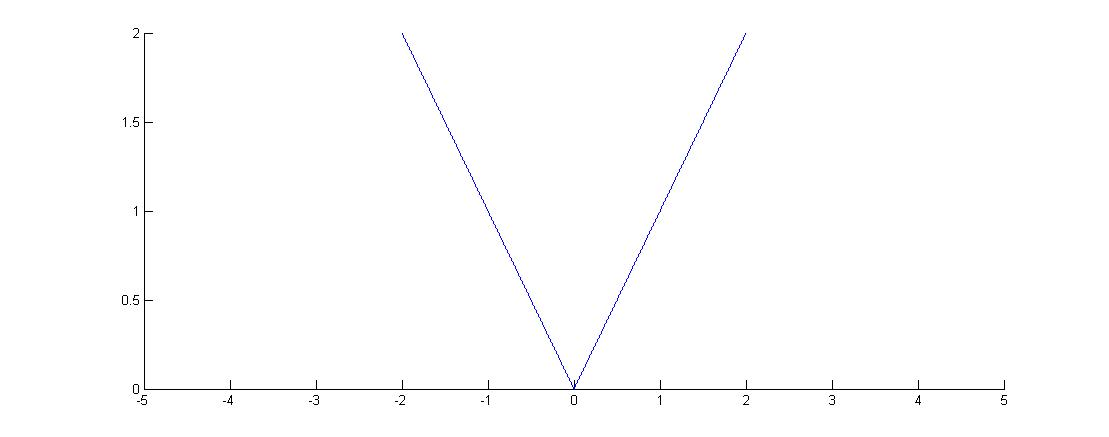
\includegraphics[width=15cm]{figures/figure8.jpg}
    }
 \end{figure}
Zusammenhang von Stetigkeit und Differenzierbarkeit:
\begin{center}
$f(x)$ differenzierbar in $x_0 \nLeftarrow f(x)$ stetig in $x_0$
\end{center}
\begin{center}
$f(x)$ differenzierbar in $x_0 \Rightarrow f(x)$ stetig in $x_0$	
\end{center}
\subsubsection*{Beispiele:}
Buch: 391\newline
Aufgabe 1
\begin{equation}
f(x)=x^3
\end{equation}
\begin{equation*}
	f'(x_0) = \lim_{\mathrm dx \to 0} \left( \frac {f(x_0 + \mathrm dx) - f(x_0)}{\mathrm dx} \right) =  
	\lim_{\mathrm dx \to 0} \left( \frac {(x_0 + \mathrm dx)^3 - (x_0)^3}{\mathrm dx} \right) =
\end{equation*}
\begin{equation*}
	\lim_{\mathrm dx \to 0} \left( \frac {(x_0^2 + 2x_0\mathrm dx + \mathrm dx^2)(x_0 + \mathrm dx) - x_0^3}{\mathrm dx} \right) =  
	\lim_{\mathrm dx \to 0} \left( \frac {(x_0^3 + 3x_0^2\mathrm dx + 3x_0\mathrm dx^2 + \mathrm dx^3) - x_0^3}{\mathrm dx} \right) =  
\end{equation*}
\begin{equation*}
	\lim_{\mathrm dx \to 0} \left( \frac { 3x_0^2\mathrm dx + 3x_0\mathrm dx^2 + \mathrm dx^3}{\mathrm dx} \right) =  
	\lim_{\mathrm dx \to 0} \left(  3x_0^2 + 3x_0\mathrm dx + \mathrm dx^2 \right) =  
\end{equation*}
\begin{equation*}
	3x_0^2 
\end{equation*}

\subsection{Ableitung der elementaren Funktionen}
Alle Ableitungen lassen sich mit Hilfe des Differenzenquotienten beweisen.
\begin{table}[h]
\begin{center}
\begin{tabular}[t]{l|l}
Funktion $f(x)$ & Ableitung $f'(x)$ \\
\hline
$f(x)=c$ & $f'(x)=0$  \\
$f(x)=x^n$ & $f'(x)=nx^{n-1}$ \\
$f(x)=\sqrt{x}=x^{\frac 12}$ & $f'(x)=\frac 12x^{-\frac 12}= \frac {1}{2\sqrt {x}}$ \\
$f(x)=\sin {x}$ & $f'(x)=\cos {x}$ \\
$f(x)=\cos {x}$ & $f'(x)=-\sin {x}$ \\
$f(x)=\tan {x}$ & $f'(x)=\frac {1}{\cos^2 {x}}$ \\
$f(x)=e^x$ & $f'(x)=e^x$ \\
$f(x)=a^x$ & $f'(x)=a^x\ln {a}$ \\
$f(x)=\ln x$ & $f'(x)= \frac 1x$ \\
$f(x)=\log_a {x}$ & $f'(x)=\frac {1}{a^x\ln {a}}$ \\
\end{tabular}
\end{center}
\label{default}
\end{table}
\subsubsection*{Beispiele}
\begin{table}[h]
\begin{center}
\begin{tabular}[t]{l|l|l}
 & Funktion $f(x)$ & Ableitung $f'(x)$ \\
\hline
a) & $f(x)=x^3$ & $f'(x)=3x^2$ \\
b) & $f(x)=2x$ & $f'(x)=2$ \\
c) & $f(x)=e^a$ & $f'(x)=0$ \\
d) &  $f(x)=\sqrt [3]{x}$ & $f'(x)=\frac 13 x^{-\frac 23} = \frac 1{3\sqrt [3]{x^2}}$ \\
\end{tabular}
\end{center}
\label{default}
\end{table}
\subsection{Ableitungsregeln von beliebigen Funktionen}
\subsubsection{Faktorregel}
\begin{equation*}
y = Cf(x)\Rightarrow y' = Cf'(x)
\end{equation*}
Beispiele
\begin{table}[h]
\begin{center}
\begin{tabular}[t]{l|l|l}
 & Funktion $f(x)$ & Ableitung $f'(x)$ \\
\hline
1) & $f(x)=5\sin {x}$ & $f'(x)=5\cos {x}$ \\
2) & $f(x)=3x^4$ & $f'(x)=12x^2$ \\
\end{tabular}
\end{center}
\label{default}
\end{table}
\subsubsection{Summenregel}
\begin{equation*}
y = f_1(x) \pm f_2(x) \pm \dotsb \Rightarrow y' = f_1'(x) \pm f_2'(x) \pm \dotsb
\end{equation*}
Beispiele
\begin{table}[h]
\begin{center}
\begin{tabular}[t]{l|l|l}
 & Funktion $f(x)$ & Ableitung $f'(x)$ \\
\hline
1) & $f(x)=5x^2 + \cos {x}$ & $f'(x)=10x -\sin {x}$ \\
2) & $f(x)=5e^x -\ln x$ & $f'(x)=5e^x - \frac 1x$ \\
\end{tabular}
\end{center}
\label{default}
\end{table}

\subsubsection{Produkteregel}
\begin{equation*}
y = f(x) * g(x) \Rightarrow y' =f'(x)*g(x) + f(x)*g'(x)
\end{equation*}
Beispiele
\begin{table}[h]
\begin{center}
\begin{tabular}[t]{l|l|l}
 & Funktion $f(x)$ & Ableitung $f'(x)$ \\
\hline
1) & $y=5x^2*\sin x$ & $f'(x)=10x$;$g'(x)=\cos x$;$y'=10x\sin x + 5x^2\cos x$ \\
2) & $y=(4x^3-3x)(2e^x-\sin x)$ & $f'(x)=12x^2-3$;$g'(x)=2e^x-\sin x$;\\
& & $y'=(12x^2-3)(2e^x-\sin x) + (4x^3 - 3x)(2e^x -\cos x)$ \\
\end{tabular}
\end{center}
\label{default}
\end{table}

\subsubsection{Quotientenregel}
\begin{equation*}
y = \frac {f(x)}{g(x)} \Rightarrow y' =\frac {f'(x)*g(x) - f(x)*g'(x)}{g^2(x)}
\end{equation*}
Beispiele
\begin{table}[h]
\begin{center}
\begin{tabular}[t]{l|l|l}
 & Funktion $f(x)$ & Ableitung $f'(x)$ \\
\hline
1) & $y=\frac {x^2}{e^x}$ & $f'(x)=2x$;$g'(x)=e^x$;$y'=\frac {2x-x^2}{e^x}$ \\
2) & $y=\frac {5x^2 + \cos x}{x^3}$ & $f'(x)=10x - \sin x$;$g'(x)=3x^2$;\\
& & $y'=\frac {(10x -\sin x)x^3-(5x^2+\cos x)3x^2}{x^6}$ \\
& & $y'=\frac {-5x^2 -x\sin x - 3\cos x}{x^4}$ \\
\end{tabular}
\end{center}
\label{default}
\end{table}

\subsubsection{Kettenregel}
\begin{equation*}
y = f(g(x)) \Rightarrow y' =f'(g(x))*g'(x)
\end{equation*}
Beispiele
\begin{table}[h]
\begin{center}
\begin{tabular}[t]{l|l|l}
 & Funktion $f(x)$ & Ableitung $f'(x)$ \\
\hline
1) & $y=\sin {5x}$ & $f'(x)=\cos x$;$g'(x)=5$;$y'=5\cos {5x}$ \\
2) & $y=e^{7x}$ & $f'(x)=e^x$;$g'(x)=7$;$y'=??$\\
3) & $y=\ln {1+x^2}$ & $f'(x)= \frac 1x$;$g'(x)=2x$;$\frac {2x}{1+x^2}$\\
4) & $y=\sqrt [3]{x^2 + 4x}$ & $f'(x)=\frac 1{3\sqrt [3]{x^2}}$;$g'(x)=2x+4$;$y'=\frac {2x+4}{3\sqrt [3]{x^2+4x}^2}$ \\
\end{tabular}
\end{center}
\label{default}
\end{table}


\subsection{Logarithmische Ableitung}
$f(x)=x^x$
\subsubsection{Logaritmieren}
\begin{equation*}
	f(x)=x^x
\end{equation*}
\begin{equation*}
	\ln {f(x)} = x \ln x
\end{equation*}
\begin{equation*}
	f'(x) \frac 1{f(x)} = \ln x + \frac xx
\end{equation*}
\begin{equation*}
	f'(x) = f(x) \ln x + f(x)
\end{equation*}
\subsubsection*{Beispiele}
\begin{equation}
	f(x) = x^{\sin x}
\end{equation}
\begin{equation*}
	\ln {f(x)} = \sin x\ln x
\end{equation*}
\begin{equation*}
	\frac 1{f(x)}f'(x)=\cos x\ln x + (\sin x)\frac 1x
\end{equation*}
\begin{equation*}
	f'(x) = \cos x\ln xx^{\sin x} + (\sin x)x^{\sin {x-1}}
\end{equation*}

\subsection{H\"ohere Ableitung}
Falls $f'(x)$ eine differenzierbare Funktion ist, so kann diese erneut abgeleitet werden und man erh\"alt $f''(x)$.\\
Durch wiederholtes differenzieren erh\"alt man die \underline{n-te Ableitung} $f^{(n)} = \frac {d^nf}{dx^n}$.
\begin{table}[h]
\begin{center}
\begin{tabular}[h]{ccccc}
$f'(x)$&$=$&$f^{(1)}(x)$&$=$&$\frac {df}{dx}$\\
$f''(x)$&$=$&$f^{(2)}(x)$&$=$&$\frac {d^2f}{dx^2}$\\
"&$=$&"&$=$&"\\
"&$=$&"&$=$&"\\
"&$=$&"&$=$&"\\
"&$=$&"&$=$&"\\
&&$f^{(n)}(x)$&$=$&$\frac {d^nf}{dx^n}$\\
\end{tabular}
\end{center}
\label{default}
\end{table}
\subsubsection*{Spezielle Notation}
$\rightarrow$ Ableitung nach der Zeit $(t)$.
\begin{equation*}
\frac {dy}{dt} = \overset {.}{y}; \frac {d^2y}{dt^2} = \overset {..}{y}
\end{equation*}

\subsection{Implizite Differentation}
Implizite Form $F(x,y)=0$.
\subsubsection*{Beispiele:}
\begin{equation*}
F(x,y)=2y^3+6x^3 +6y-24x=0
\end{equation*}
Steigung gegen\"uber der x-Achse?
\begin{itemize}
\item Gliderweise ableiten nach x, wobei y=y(x) ebenfalls abgeleitet werden muss
\item Aufl\"osen nach $y'$
\item gegebene Stellen $(x_0,y_0)$ einsetzen (falls die Steigung in einem Punkt gesucht ist)
\end{itemize}
\subsubsection*{Beispiele}
\begin{equation}
F(x,y)=2y^3+6x^3+6y-24x=0
\end{equation}
\begin{equation*}
\frac {dF}{dx} = 6y^2y' + 18x^2 + 6y' -24=0
\end{equation*}
\begin{equation*}
y'(6y^2+6)+18x^2-24=0
\end{equation*}
\begin{equation*}
y'(6y^2+6)=24-18x^2
\end{equation*}
\begin{equation*}
y'= \frac {6(4-3x^2)}{6(y^2+1)}=\frac {4-3x^2}{y^2+1}
\end{equation*}
Steigung im Punkt $(0,0)$ gegen\"uber der x-Achse.
\begin{equation*}
y'(0,0)=4
\end{equation*}

\subsection{Ableitung einer Kurve in Parameterform}
\begin{equation*}
\left\lbrace \begin{array}{ccc}
  x & = & x(t)\\
  y & = & y(t)\\
\end{array}\right\rbrace
\text{Parameterdarstellung einer Kurve.}
\end{equation*}
\begin{equation*}
y'=\frac {dy}{dt} * \frac {dt}{dx} = \frac {dy}{dx} = \frac {\overset {.}{y}}{\overset {.}{x}}
\end{equation*}
\subsection{Tangenten- und Normalengleichung / Linearisierung von Funktionen}
\begin{figure}[h]
  \centering
  \fbox{
    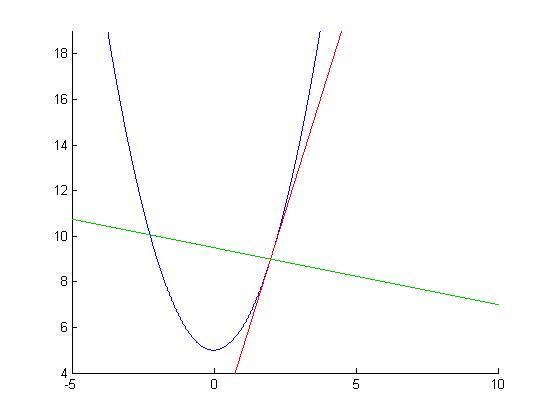
\includegraphics[width=15cm]{figures/figure9.jpg}
    }
 \end{figure}
 $f'(x)$ Steigung\\
 $(x_0,y_0)$ Ber\"uhrungspunkt\\
 $(x,y)$ beliebiger Punkt auf der Tangente
 \subsubsection{Tangentengleichung}
\begin{figure}[h]
  \centering
 \fbox{
 	$\frac {y-y_0}{x-x_0} = f'(x_0)$ 
 }
  \end{figure}
 Jeder Punkt $(x,y)$ auf der Tangente erf\"ullt die Tangentengleichung.
 \subsubsection{Normalengleichung}
\begin{figure}[h]
  \centering
 \fbox{
	$\frac {y-y_0}{x-x_0} = -\frac 1{f'(x_0)}$
 }
  \end{figure}

 Mit Hilfe der Tangentengleichung kann eine Funktion \underline{linearisiert} werden. Das heisst sie wird \underline{lokal} durch eine \underline{lineare Funktion approximiert}(angen\"ahert).\\
 Durch Umformen der \underline{Tangentengleichung} erhalten wir diese lineare Funktion.\\
 Allgemeine Form einer linearen Funktion
 \begin{equation*}
 y=ax+b
 \end{equation*}
 Das heisst die Tangentengleichung muss nach $y$ aufgel\"ost werden.
 \begin{equation*}
 \frac {y-y_0}{x-x_0}=f'(x) \Rightarrow y=f'(x_0)(x-x_0)+y_0
 \end{equation*}
\begin{figure}[h]
  \centering
  
  \fbox{
  $y=f'(x_0)x-f'(x_0)x_0 + y_0$
 }

  \end{figure}
 \subsubsection*{Beispiele:}
 \begin{equation}
 f(x)=x^2-2x+1; P(x_0,y_0)=(0,1)
 \end{equation}
 \begin{equation*}
 f'(x)=2x-2
 \end{equation*}
 Linearisierung der Funktion
 \begin{equation}
 y=(2x_0-2)x+-(2x_0-2)x_0+y_0
 \end{equation}
 \begin{equation*}
 y=-2x+1
 \end{equation*}
 
 \subsection{Charakteristische Kurvenpunkte}
 Charakteristische Kurvenpunkte bestimmen das Aussehen der Kurve.\\
 Charakteristische Kurvenpunkte sind:\\
 \begin{itemize}
 	\item Nullstellen
	\item Maxima
	\item Minima
	\item Wendepunkte
	\item Sattelpunkte
\end{itemize}
\underline{Vorbereitung:} Geometrische Bedeutung von $f'(x)$ und $f''(x)$\\\\
\underline{1. Ableitung:} \\
	\begin{table}[h]
		\begin{center}
			\begin{tabular}[h]{c|c|c}
				&&Tangente \\
				\hline
				$f'(x_0)\rangle 0$&$f(x)$ ist in $x_0$ wachsend & wachsend \\
				$f'(x_0) \langle 0$&$f(x)$ ist in $x_0$ fallend & fallend \\
				$f'(x_0) = 0$& / & waagrecht\\
			\end{tabular}
		\end{center}
		\label{default}
	\end{table}
	\\
\underline{2. Ableitung}\\
	\begin{table}[h]
		\begin{center}
			\begin{tabular}[h]{c|c|c}
				&&Kr\"ummung \\
				\hline
				$f''(x_0)\rangle 0$&$f'(x)$ ist in $x_0$ wachsend & linkskr\"ummung \\
				$f''(x_0) \langle 0$&$f'(x)$ ist in $x_0$ fallend & rechtskr\"ummung \\
				$f''(x_0) = 0$& / & weder links- nocht rechtskr\"ummung\\
			\end{tabular}
		\end{center}
		\label{default}
	\end{table}
\\
\underline{Nullstellen:} \\
	\begin{center}
		$f(x)=0$
	\end{center}

\underline{Maxima:} \\
	\begin{center}
		$f'(x)=0$ und $f''(x) \langle 0$
	\end{center}

\underline{Minima:} \\
	\begin{center}
		$f'(x)=0$ und $f''(x) \rangle 0$
	\end{center}
\underline{Wendepunkt:} \\
	\begin{center}
		$f'(x)\neq0$ und $f''(x)= 0$ und die Kr\"ummungen links und rechts von $x_0$ sind unterschiedlich, also Vorzeichenwechsel von $f''(x)$
	\end{center}
\underline{Sattelpunkt:} \\
	\begin{center}
		$f'(x)=0$ und $f''(x)= 0$ und die Kr\"ummungen links und rechts von $x_0$ ist identisch
	\end{center}
\underline{Bemerkung: } (Wende-/Sattelpunkt)\\
	\begin{equation*}
		f(x)=x^4
	\end{equation*}
	\begin{equation*}
		f'(x)=4x^3
	\end{equation*}
	\begin{equation*}
		f''(x)=12x^2
	\end{equation*}
	\newpage
	\begin{center}
		Wir betrachten den Punkt $(0,0)$
		\begin{figure}[h]
		\fbox{
    			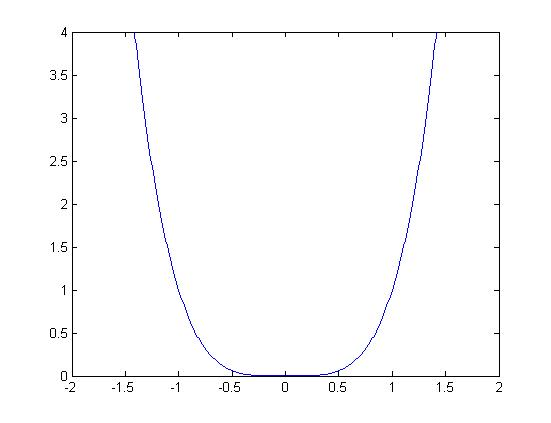
\includegraphics[width=10cm]{figures/figure11.jpg}
		}
	 \end{figure}
	\end{center}
	\begin{equation*}
		\left\lbrace \begin{array}{ccc}
			  f'(0) & = & 0\\
			  f''(0) & = & 0\\
		\end{array}\right\rbrace 
		\Rightarrow \text{Sattelpunkt}\Rightarrow \text{Wiederspruch zum Graph}
	\end{equation*}
	%\begin{equation*}
	%	\Rightarrow \text{Wiederspruch zum Graph}
	%\end{equation*}
	\begin{equation*}
		\Rightarrow 
		\text {2. Ableitung } f''(x)=0 \text{ reicht nicht aus}
	\end{equation*}
\underline{Anmerkung:}\\
	Anstelle des Vorzeichenwechsels von $f''(x)$ kann auch die \underline{dritte Ableitung} von $f(x)$ betrachtet werden. Es muss gelten:
	\fbox{
		$f'''(x)\neq0$
	}\\
\underline{Problem:}\\
	$f'''(x)=0$: Keine Aussage m\"oglich\\
	Es reicht, wenn irgendeine ungerade Ableitung ungleich 0 ist, damit wir einen Wendepunkt habe.\\
\underline{Beispiele:}\\
	\begin{equation}
		f(x)=x^4-x^3-3x^2+5x-2
	\end{equation}
	\begin{table}[h]
		\begin{center}
			\begin{tabular}[h]{ll}
				\underline{Nullstellen:} &$x=\lbrace 1, -2\rbrace$\\
				\underline{Maxima:} & $x=\lbrace \rbrace$\\
				\underline {Minima:} & $x=\lbrace-\frac 54 \rbrace$\\
				\underline{Wendepunkte:} & $x=\lbrace-\frac 12 \rbrace$\\
				\underline{Sattelpunkte:} & $x=\lbrace 1 \rbrace$\\
			\end{tabular}
		\end{center}
		\label{default}
	\end{table}
	\newpage
	\underline{Zusammengefasst:}\\
	\begin{table}[h]
		\begin{center}
			\begin{tabular}[h]{ll}
				\underline{Nullstellen:} & $(1,0), (-2,0)$\\
				\underline{Maxima:} & \\
				\underline {Minima:} & $\left(-\frac 54,f(-\frac 54)\right)=(-\frac 54, -\frac {17}{2})$\\
				\underline{Wendepunkte:} & $\left(-\frac 12, f(-\frac 12)\right)=(-\frac 12, -5.06)$\\
				\underline{Sattelpunkte:} & $(1,0)$\\
				\underline{Graph(Skizze):} & \\
			\end{tabular}
		\end{center}
		\label{default}
	\end{table}
	\begin{figure}[h]
		\fbox{
    			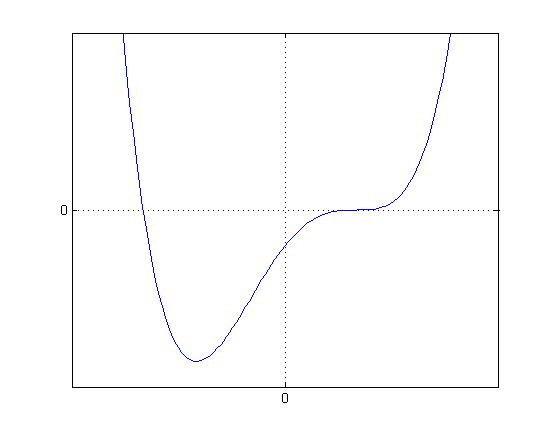
\includegraphics[width=10cm]{figures/figure10.jpg}
		}
	 \end{figure}\newpage
\subsection{Extremwertaufgaben}
Mit Hilfe der ersten Ableitung k\"onnen wir die \underline{Extremalstellen} einer Funktion bestimmen. Diese Tatsache k\"onnen wir verwenden, um verschiedenste Problemstellungen zu l\"osen, in welchen eine Gr\"osse \underline{maximiert} oder \underline{minimiert} werden soll, wenn es uns gelingt die gesuchte Gr\"osse als Funktion auszudr\"ucken.
\subsubsection*{Beispiel:}
Ein 40 cm langes St\"uck Draht soll zu einem Rechteck von maximalem Fl\"acheninhalt geformt werden. Wie lange sind die Seiten des Rechtecks zu w\"ahlen?
\begin{equation}
	2x+2y=40 cm
\end{equation}
\begin{equation*}
	F(x,y)=x*y
\end{equation*}
\begin{equation*}
	f(x)=-x^2+20x \Rightarrow f'(x)=0 \Rightarrow x= 10 = y
\end{equation*}
\subsubsection*{Allgemeines Vorgehen}
\begin{itemize}
\item festlegen der Variablen
\item Die zu optimierende/minimierende Gr\"osse durch diese Variablen ausdr\"ucken
\item Der Ausdruck f\"ur diese Gr\"osse auf eine Variable reduzieren unter Verwendung der Nebenbedingung(en)
\item Ausruck ableiten und null setzen
\item L\"osung bestimmen
\end{itemize}
\newpage
\section{Integralrechnung}
\subsection{Integration als Umkehrung der Differentation}
\begin{equation*}
	f(x)\xrightarrow{\text{Differentation}} f'(x)
\end{equation*}
\begin{equation*}
	f(x)\xleftarrow[\text{Integration}]{} f'(x)
\end{equation*}
\subsubsection*{Beispiel 1:}
\begin{equation*}
	f'(x) = 1
\end{equation*}
\begin{equation*}
	\Rightarrow f(x) = x + C 
\end{equation*}	
	$\text{S\"amtliche Funktionen welche abgeleitet 1 ergeben ($C=$ Integrationskonstante)}$
\subsubsection*{Graphik (Kurvenschar)} Insert from Matlab 
\subsubsection*{Beispiel 2:}
\begin{equation*}
	y' = 2x
\end{equation*}
\begin{equation*}
	\Rightarrow y = x^2 + C
\end{equation*}
\subsubsection*{Definition:}
Eine Funktion $F(x)$ heisst \underline{Stammfunktion} zu $f(x)$, wenn gilt:
\fbox{
		F'(x) = f(x)
}
\subsubsection*{Bemerkung:}
Zu jeder Funktion gibt es unendliche viele Stammfunktionen.
\subsubsection*{Beispiele:}
\begin{equation}
	f(x)=2x \Rightarrow F(x) = x^2 + C \text{, da } F'(x) = f(x)
\end{equation}
\begin{equation}
	f(x)=\sin x  \Rightarrow F(x) = -\cos x + C 
\end{equation}
\begin{equation}
	f(x)=4x^3 \Rightarrow F(x) = x^4 + C 
\end{equation}
\begin{equation}
	f(x)=x^a \Rightarrow F(x) = \frac {1}{a+1}*x^{a+1}+C
\end{equation}
\begin{equation}
	f(x)=5x^2 \Rightarrow F(x) = \frac {5}{3}*x^{3}+C
\end{equation}
\subsubsection*{Definition}
Das Aufsuchen \underline{s\"amtlicher} Stammfunktionen einer vorgegebenen Funktion $f(x)$ wird als \underline{Integration} bezeichnet.
\subsection{Das bestimmte Integral als Fl\"acheninhalt}
Insert graph from matlab
\subsubsection*{Idee:} wir teilen das Fl\"achenst\"uck in Streifen und summieren die Fl\"achen\newline
Insert graph from matlab\newline
Jeder Streifen wird in geeigneter Weise durch ein Rechteck ersetzt.
\begin{table}[h]
	\begin{center}
		\begin{tabular}[h]{c|c}
			\underline{Untersumme}&\underline{Obersumme}\\
			\hline
			Insert Graph & Insert Graph\\
			$U_5 = f(x_0)*\Delta x_1 +  f(x_1)*\Delta x_2 +$ & $O_5 = f(x_1)*\Delta x_1 +  f(x_2)*\Delta x_2 +$ \\
			\indent $\cdots + f(x_4)*\Delta x_5$& \indent $ \cdots + f(x_5)*\Delta x_5$\\
			$U_5 = \sum\nolimits_{k=1}^5 f(x_{k-1})*\Delta x_k$       & $O_5 = \sum\nolimits_{k=1}^5 f(x_{k})*\Delta x_k$\\
			$U_5 = 2.04$& $O_5 = 2.64$\\
		\end{tabular}
	\end{center}
\end{table}
Je feiner die Streifen gew\"ahlt werden, desto genauer die Berechnung.\newline
Sei $n$ die Anzahl Streifen, in welche das Interval [1,2] geteilt wird. So gilt f\"ur $n \to \infty$\newline
\begin{center}
	$U_n \to A$\newline
	$O_n \to A$\newline
\end{center}
folglich:
\begin{equation*}
	A = \lim_{n \to \infty} U_n = \lim_{n \to \infty} O_n = \lim_{n \to \infty} \sum_{k=1}^n f(x_k)*\Delta x_k
\end{equation*}
\begin{equation*}
	\doteq \int_{1}^2 f(x)\,dx = F(2)-F(1)
\end{equation*}
\begin{equation*}
	\int_{1}^2 x^2\,dx =  \frac 13 x^3\vert_1^2 = \frac 83 - \frac 13 = \frac 73 = 2.\overline{33}
\end{equation*}
\subsubsection*{Allgemein:}
\begin{equation*}
	A = \int_{a}^b f(x)\,dx =  F(x)\vert_a^b = F(b) - F(a)
\end{equation*}

\subsection{Uneigentliche Integrale}
Uneigentliche Integrale sind Integrale der Form
\begin{equation*}
	\int_{-\infty}^\infty f(x)\,dx , \int_{-\infty}^b f(x)\,dx , \int_{a}^\infty f(x)\,dx 
\end{equation*}
\subsubsection*{Berechnung:}
\begin{itemize}
\item[1] Ersetze $\pm\infty$ durch $\lambda$
\item[2] Berechene $\lim_{\lambda \to \infty} \int_a^\lambda f(x)\,dx$\newline
	Ist das Integral beschr\"ankt, so ist es \underline{konvergent}, andernfalls \underline{divergent}
\end{itemize}
\subsubsection*{Beispiel:}
\begin{equation*}
	\int_{-\infty}^0 e^x \,dx = \lim_{\lambda \to \infty} \int_{-\lambda}^0 e^x \,dx = \lim_{\lambda \to \infty} 	
	e^x \vert_{-\lambda}^0 = \lim_{\lambda \to \infty} e^0-e^{-\lambda} = 1
\end{equation*}
\subsection{Integrationsregeln}
\subsubsection{Faktorregel:}
\begin{equation*}
	\int_a^b c*f(x)\,dx = c * \int_a^b f(x) \,dx
\end{equation*}
\subsubsection{Summenregel:}
\begin{equation*}
	\int_a^b f(x)\pm g(x)\,dx = \int_a^b f(x) \,dx \pm \int_a^b g(x) \,dx
\end{equation*}
\subsubsection{Vertauschregel:}
\begin{equation*}
	\int_a^b f(x)\,dx = - \int_b^a f(x) \,dx
\end{equation*}
\subsubsection{Nullintegral:}
\begin{equation*}
	\int_a^b c*f(x)\,dx = 0, \text{ f\"ur } a=b
\end{equation*}
\subsubsection{Zerlegung:}
\begin{equation*}
	\int_a^b c*f(x)\,dx = \int_a^c f(x) \,dx + \int_c^b f(x) \,dx, \text{ f\"ur } a \leq c\leq b
\end{equation*}

\subsection{Integrationsmethoden}
\subsubsection{Integration durch Substitution}
\begin{equation*}
	\text{Beispiel: } \int x*\cos(x^2)\,dx \text{ ist kein Grundintegral}
\end{equation*}
Mit Hilfe der Substitution l\"asst es sich aber in ein Grundintegral verwandeln, welches wir integrieren k\"onnen.\newline
Unter \underline{Substitution} versteht man das Ersetzen eines Ausdrucks durch einen anderen (geeigneteren).\newline
Wir ersetzen also $x^2$ druch $u \Rightarrow u=x^2$.\newline
$dx$ wird ebenfalls ersetzt.
\begin{equation*}
	\frac {du}{dx} = 2x \text{, da } u=x^2 \Rightarrow dx = \frac {du}{2x}
\end{equation*}

\begin{equation*}
	\Rightarrow \int x*\cos(u)* \frac {du}{2x} \,
\end{equation*}
somit
\begin{equation*}
	\int \cos(u)* \frac 1{2} \,du = \frac 12 \sin(u) + C
\end{equation*}
Nun wird dieses $u$ wieder zur\"uckersetzt (R\"ucksubstitution)
\begin{equation*}
		\Rightarrow \frac 12 \sin(x^2) + C
\end{equation*}
\underline{Allgemein:}
\begin{equation*}
	u = g(x)
\end{equation*}
\begin{equation*}
	\frac {du}{g'(x)} = dx
\end{equation*}
\begin{equation*}
	\text{Integration nach } u
\end{equation*}
\begin{equation*}
	\text{R\"ucksubstitution} g(x) =u
\end{equation*}
Was wenn Integrationsgrenzen vorhanden sind?
\begin{equation*}
	\int_0^\pi (\cos(x))^3*\sin(x)\,dx
\end{equation*}
\begin{equation*}
	\text{Substitution} \cos(x) =u, \frac {du}{dx} = -\sin(x) \Rightarrow dx = \frac{du}{-\sin(x)}
\end{equation*}
\begin{equation*}
	\int_?^? u^3*\sin(x)\,\frac{du}{-\sin(x)} = 	\int_?^? u^3\,du
\end{equation*}
\begin{equation*}
	0,\pi \text{ entsprechen den Grenzen f\"ur } x
\end{equation*}
\begin{equation*}
	\Rightarrow \cos(0),\cos(\pi) \text{ entsprechen den Grenzen f\"ur } u \text{, da } u = \cos(x)
\end{equation*}
\underline{Allgemein:}
\begin{equation*}
	u = g(x)
\end{equation*}
\begin{equation*}
	\frac {du}{g'(x)} = dx
\end{equation*}
\begin{equation*}
	\text{Integrationsgrenzen } g(x),g(x)
\end{equation*}
\begin{equation*}
	\text{Integration nach } u
\end{equation*}
\begin{equation*}
	\text{Integral berechnen R\"ucksubstitution f\"allt weg}
\end{equation*}
\subsubsection{Partielle Integration}
Der Integrand $f(x)$ des vorgegebenen Integrals $\int f(x)\,dx$ wird zun\"achst in geeigneter Weise in ein Produkt einer Funktion $u(x)$ und der Ableitung $v'(x)$ einer Funktion $v(x)$ zerlegt.
\begin{equation*}
	\Rightarrow \int f(x)\,dx = \int u(x)*v'(x)\,dx
\end{equation*}
Das Integral l\"asst sich dann folgendermassen darstellen: (Formel der partiellen Integration)
\begin{equation*}
	\int f(x)\,dx = \int u(x)*v'(x)\,dx = u(x)v(x) - \int u'(x)*v(x)\,dx
\end{equation*}

\section{Anwendungen der Integralrechnung}
\subsection{Fl\"achenberechnung}
\subsubsection*{Fallunterscheidung:}
\begin{itemize}
	\item[a)] $f(x)\geq 0$, $\int_a^b f(x)\,dx$ beschreibt die Fl\"ache, Beispiel: $f(x)=-x^2+10$
	\item[b)] $f(x)\geq 0$ und $f(x)$ strebt gegen \underline{null}, Beispiel: $f(x)=e^x$\newline 
		$\int_{-\infty}^\infty f(x)\,dx , \int_{-\infty}^b f(x)\,dx , \int_{a}^\infty f(x)\,dx $	\newline
		Das \underline{uneigentliche} Integral bestimmt den Fl\"acheninhalt.
	\item[c)] $f(x) \leq 0$ $ \int_a^b f(x) \,dx \leq 0 \Rightarrow$ Fl\"ache $= \vert \int_a^b f(x) \,dx \vert 			\geq 0$ , Beispiel: $f(x)=x^2-10$
	\item[d)] $f(x) \geq 0 \land f(x) \leq 0$, Beispiel: $f(x)=\sin(x)$\newline
		$\int_a^b f(x) \,dx = \vert\int_a^c f(x) \,dx \vert + \vert \int_c^b f(x) \,dx \vert$ (falls c die einzige Nullstelle ist)
	\item[e)] Fl\"ache zwischen zwei Kurven\newline
		$A = \int_a^b f(x)-g(x)\,dx \rightarrow$ Lage der Fl\"achen ist egal
\end{itemize}
\subsection{Bogenl\"ange einer ebenen Kurve}
\begin{equation*}
	B \sim \sum_{ds} ds
\end{equation*}
\begin{equation*}
	ds = \sqrt{(dx)^2 + (dy)^2} = \sqrt{(dx)^2 + (dy)^2 * \frac{(dx)^2}{(dx)^2}} = 
\end{equation*}
\begin{equation*}
	\sqrt{(dx)^2 + (dx)^2 * \frac{(dy)^2}{(dx)^2}} = dx* \sqrt{ 1 +  \frac{(dy)^2}{(dx)^2}}
\end{equation*}
\begin{equation*}
	ds = dx* \sqrt{ 1 +  (f'(x))^2}
\end{equation*}
\newline
\begin{equation*}
	B = \lim_{ds \to 0} \sum_{ds} ds = \lim_{dx \to 0} \sum_{dx} \sqrt { 1 +  (f'(x))^2} *dx
\end{equation*}
\begin{equation*}
	B = \int_a^b \sqrt { 1 +  (f'(x))^2} \,dx
\end{equation*}
\subsubsection*{Beispiel (Kreisumfang):}
\begin{equation*}
	\text{Kreisgleichung: } r^2 = y^2+x^2
\end{equation*}
\begin{equation*}
	y = \sqrt {r^2-x^2}
\end{equation*}
\begin{equation*}
	B = \int_a^b \sqrt { 1 +  (f'(x))^2} \,dx
\end{equation*}
\begin{equation*}
	\frac 14 U = \int_0^r \sqrt { 1 +  (y')^2} \,dx
\end{equation*}
\begin{equation*}
	y' = \frac 12 * \frac {-2x}{\sqrt{r^2-x^2}} = - \frac {x}{\sqrt{r^2-x^2}}
\end{equation*}
\begin{equation*}
	(y')^2 = \frac {x^2}{r^2-x^2}
\end{equation*}
\begin{equation*}
	\frac 14 U =\int_0^r \sqrt{ 1+\frac {x^2}{r^2-x^2} }\,dx = \int_0^r \sqrt{ \frac {r^2}{r^2-x^2} }\,dx = \int_0^r \frac{r}{\sqrt{r^2-x^2}}\,dx
\end{equation*}
\newline Substitution
\begin{equation*}
	x = r * \sin (u) \Rightarrow u = \arcsin \left( \frac xr\right)
\end{equation*}
\begin{equation*}
	\frac{dx}{du} = r * \cos (u) \Rightarrow dx = r*\cos (u) * du
\end{equation*}
\begin{equation*}
	\int_{\arcsin \frac 0r}^{\arcsin \frac rr} \frac r{\sqrt{r^2-r^2* \sin^2 (u)}} * r *\cos (u) \,du =
\end{equation*}
\begin{equation*}
	\int_{0}^{\frac \pi2} \frac r{\sqrt{r^2*(1- \sin^2 (u)}} * r *\cos (u) \,du =
\end{equation*}
\begin{equation*}
	\int_{0}^{\frac \pi2} \frac r{\sqrt{r^2*\cos^2 (u)}} * r *\cos (u) \,du =
\end{equation*}
\begin{equation*}
	\int_{0}^{\frac \pi2} \frac r{r*\cos (u)} * r *\cos (u) \,du =
\end{equation*}
\begin{equation*}
	\int_{0}^{\frac \pi2} r \,du = ru \vert_0^{\frac \pi2} = \frac {\pi*r}2
\end{equation*}
\begin{equation*}
	\frac 14 U =  \frac {\pi*r}2 \Rightarrow U = 2*\pi*r
\end{equation*}
\subsection{Rotationsk\"orper}
\begin{equation*}
	V = \pi*r^2 * h
\end{equation*}
\begin{equation*}
	\text{W\"ahle: }r = f(x), h = dx
\end{equation*}
\begin{equation*}
	\text{Summiere: }\lim_{dx \to 0} \pi * \sum_{dx} f^2(x) dx \Rightarrow \pi \int_a^b f^2(x) \,dx
\end{equation*}

\subsection{Mantelfl\"ache}
\begin{equation*}
	M = 2\pi*r* S
\end{equation*}
\begin{equation*}
	\text{W\"ahle: }r = f(x), S = \sqrt{dx^2-dy^2}
\end{equation*}
\begin{equation*}
	\text{Summiere: }\lim_{dx \to 0} 2\pi * \sum_{dx} f(x)* \sqrt{1+f'(x)} dx \Rightarrow 2\pi \int_a^b f(x)*\sqrt{1+f'(x)} \,dx
\end{equation*}



\newpage 
\printindex
\end{document}  
